\documentclass{beamer}

\usepackage{mathtools}

\usepackage{xcolor}

\usepackage{tikz}
\usetikzlibrary{positioning,arrows}

\usepackage{xcolor}
\definecolor{YaleBlue}{HTML}{00356B}

\usetheme{Rochester}
\usecolortheme[named=YaleBlue]{structure}
\beamertemplatenavigationsymbolsempty{}
\setbeamercovered{transparent}

\graphicspath{{images/}}

\newenvironment{itemize+}{\begin{itemize}[<+->]}{\end{itemize}}

\date{}

\title{Epistatic effects among lung adenocarcinoma somatic mutations
  across oncogenesis} \author{Jorge Alfaro-Murillo, Krishna Dasari \&
  Jeffrey Townsend}
\institute{Biostatistics Department\\
  
\includegraphics[height=0.7in]{ysph}}

\begin{document}

\begin{frame}[plain]
  \maketitle
\end{frame}

\begin{frame}
  \frametitle{Motivation}
  \begin{itemize+}
  \item \textit{KRAS} and \textit{TP53} are considered early drivers
    of LUAD but which is first?
  \item Smoking causes LUAD but is it just because of more mutations?
  \item Why is \textit{EGFR} in so many non-smoker LUAD cases?
  \end{itemize+}
\end{frame}

\begin{frame}
  \frametitle{Model}

  \begin{itemize+}
  \item There is a constant rate at which mutations occur and are
    selected to high frequency (flux)
  \item The flux depends on the gene that will mutate as well as the
    current somatic genotype (previous mutations)
    \begin{center}
      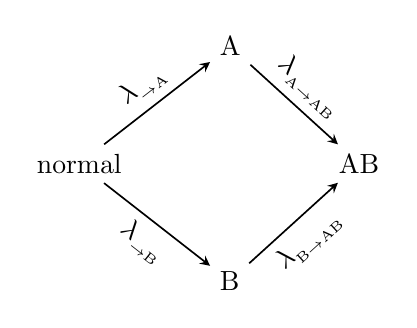
\begin{tikzpicture}[arrow/.style={-stealth,semithick}]
        \node (wt) {normal}; \node (m10) [above right=of wt] {$\mathrm{A}$}; \node
        (m01) [below right=of wt] {$\mathrm{B}$}; \node (m11) [below right=of
        m10] {$\mathrm{AB}$}; \draw[arrow] (wt) to node [sloped, above]
        {$\lambda_{{}_{\varnothing\rightarrow\mathrm{A}}}$} (m10); \draw[arrow] (wt) to node [sloped,
        below] {$\lambda_{{}_{\varnothing\rightarrow\mathrm{B}}}$} (m01); \draw[arrow] (m01) to node
        [sloped, below] {$\lambda_{{}_{\mathrm{B}\rightarrow \mathrm{AB}}}$} (m11);
        \draw[arrow] (m10) to node [sloped, above]
        {$\lambda_{{}_{\mathrm{A}\rightarrow \mathrm{AB}}}$} (m11);
      \end{tikzpicture}
    \end{center}
    \item Epistasis occurs when
      $\lambda_{\varnothing\rightarrow\mathrm{A}} \neq
      \lambda_{B\rightarrow\mathrm{AB}}$
    \item Given the number of tumors in each genotype we can estimate
      the fluxes
    \end{itemize+}
\end{frame}


\begin{frame}
  \frametitle{Deconvolution of mutation and selection}
  \begin{itemize+}
  \item The flux is deconvolved into the mutation rate of the gene and
    the strength of selection on mutations of gene
  \item Mutation rate are obtained for each possible variant of each
    gene considering:
    \begin{itemize}
    \item Molecular signatures
    \item Gene expression
    \item Chromatin marks
    \item Replication times
    \end{itemize}
  \end{itemize+}
\end{frame}


\begin{frame}
  \frametitle{Epistasis in most commonly mutated genes in TCGA}
  \begin{center}
    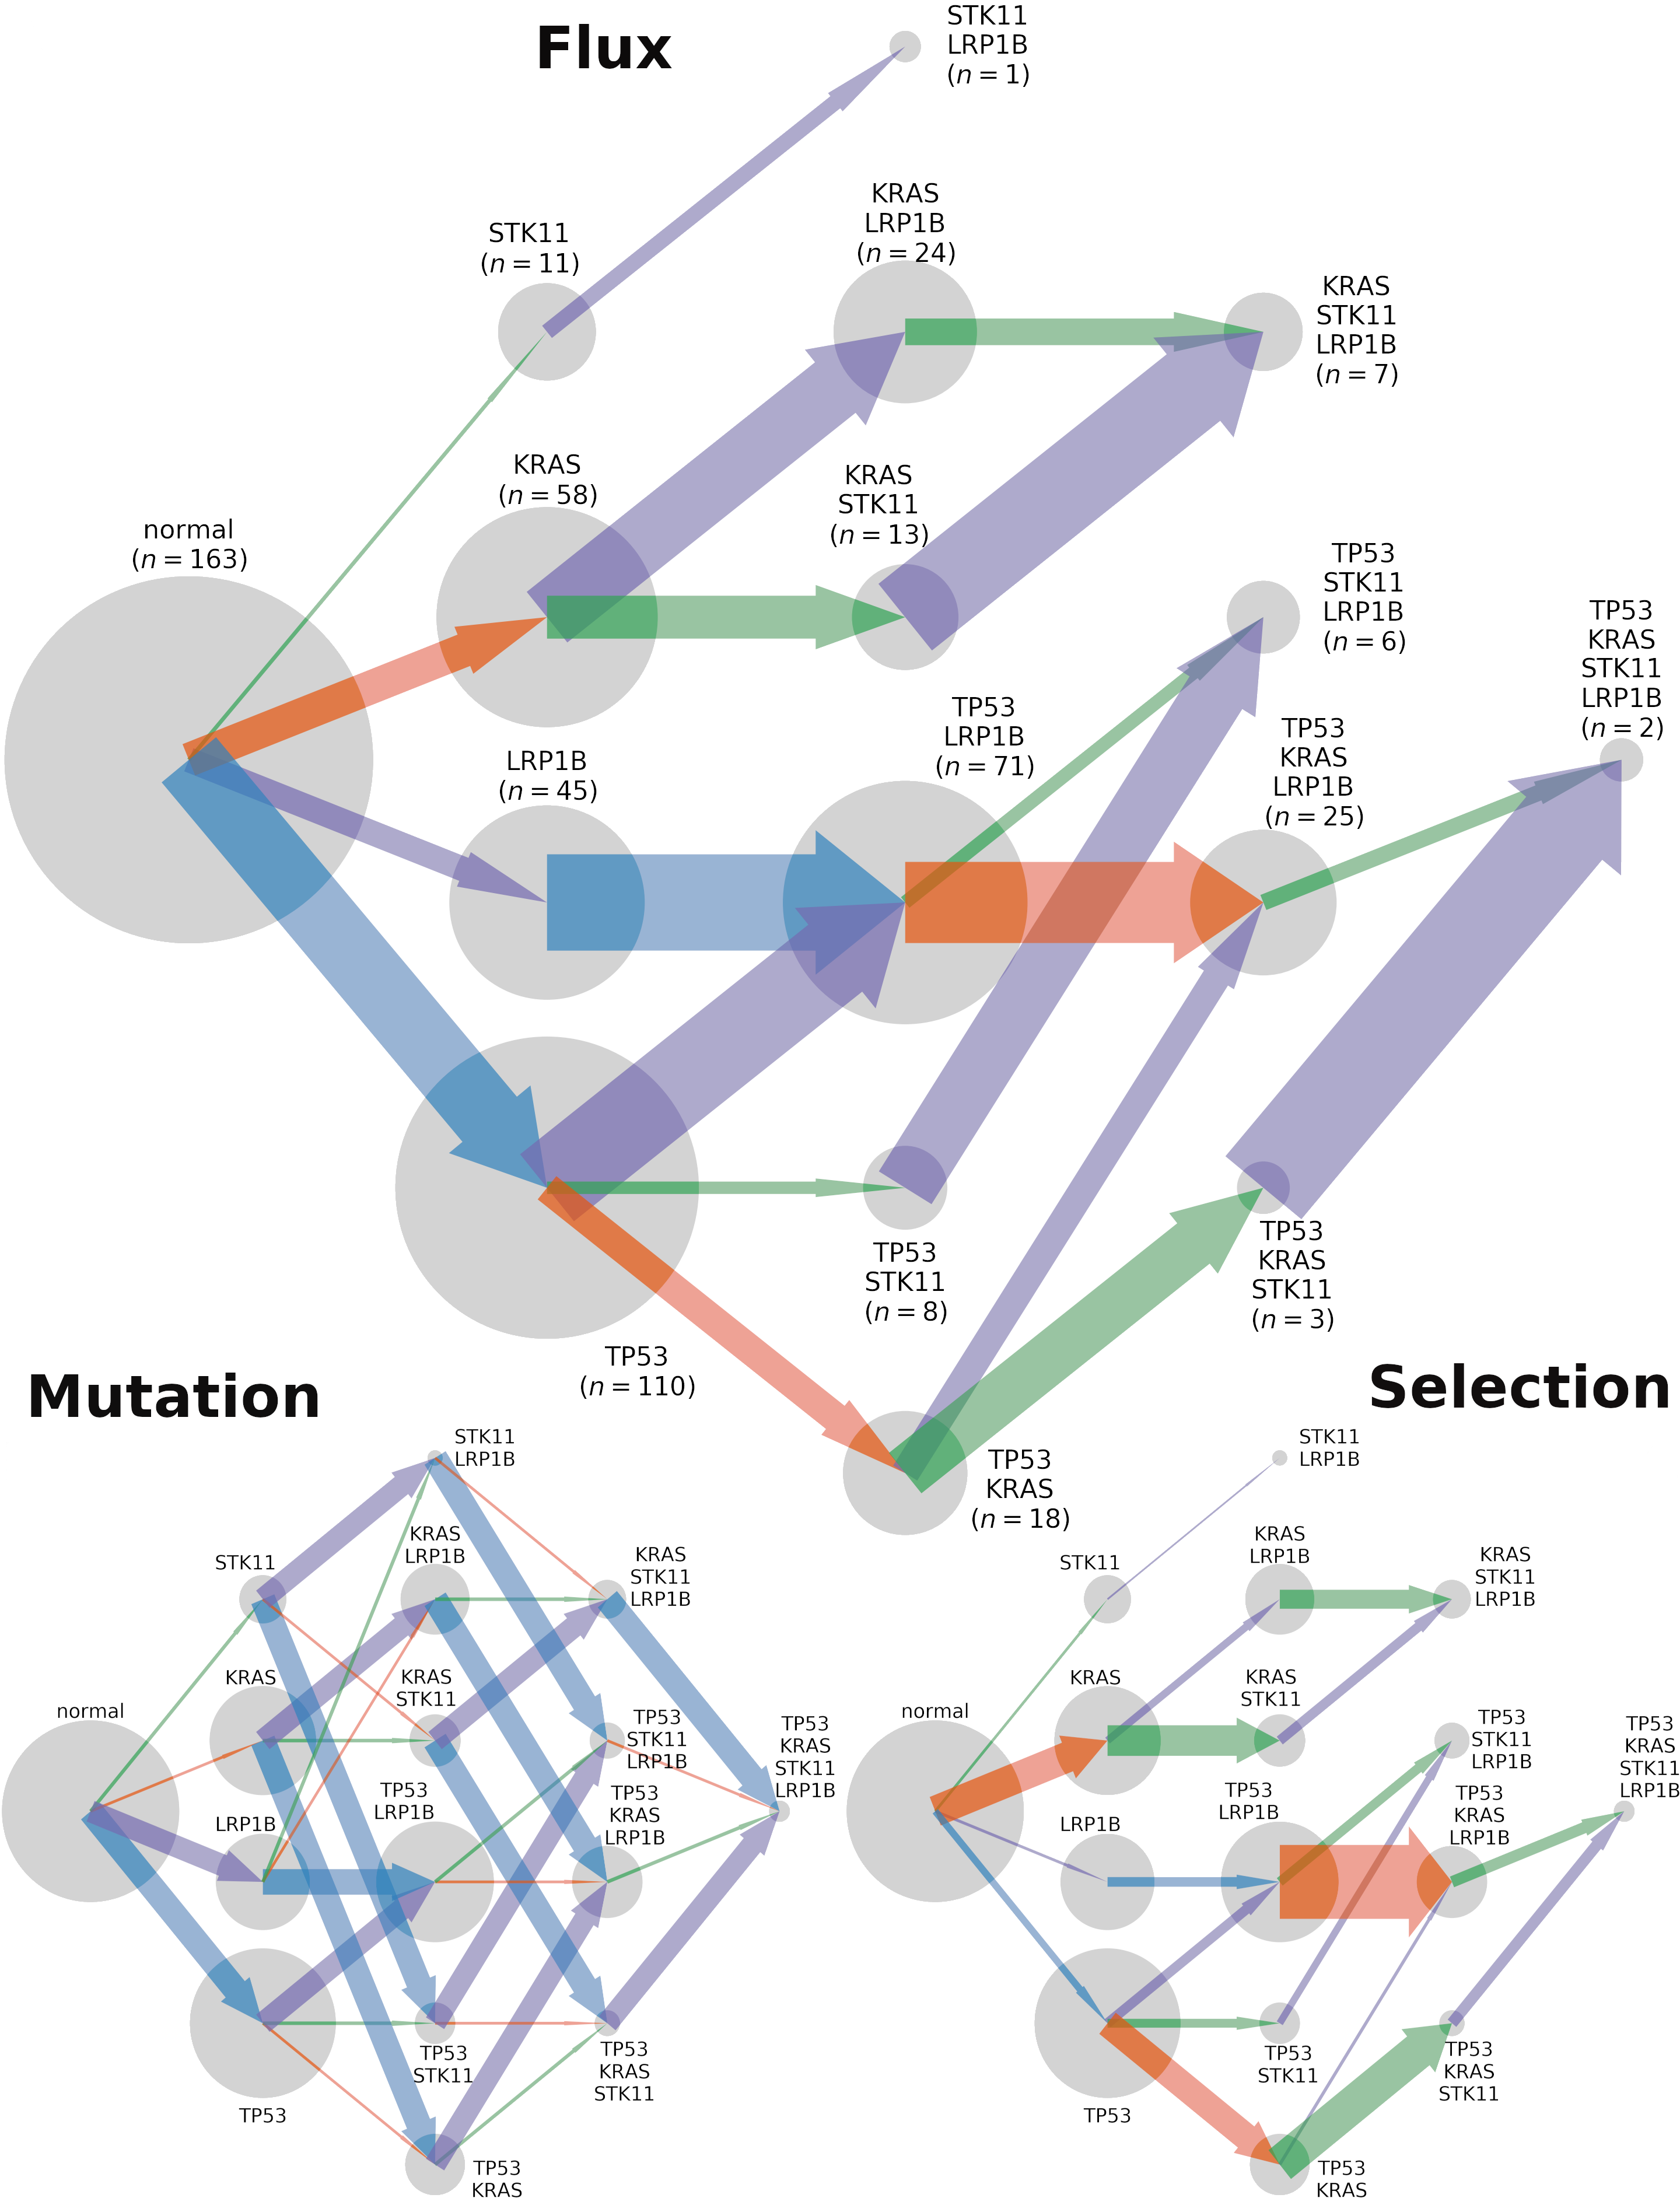
\includegraphics[height=3in]{all_landscapes_luad_4_sf}
  \end{center}
\end{frame}

\begin{frame}
  \frametitle{Larger data set}
  \begin{itemize}
  \item How about other genes? What is the effect of smoking? \pause
  \item Aggregate multiple data

    \begin{enumerate}
    \item The Cancer Genome Atlas (TCGA)
    \item AACR Project GENIE
    \item Kenfield et al. Tob Control, 2008
    \item Chen et al. Nat Genet, 2020
    \item Rizvi et al. Science, 2015
    \item Hellmann et al. Cancer Cell, 2018
    \item Jamal-Hanjani et al. N Engl J Med, 2017
    \item Abbosh et al. Nature, 2017
    \item Imielinski et al. Cell, 2012
    \item Ding et al. Nature, 2008
    \item Jordan et al. Cancer Discov, 2017
    \end{enumerate}\pause
  \item Total: 8,487 non-metastatic LUAD samples \pause
  \item Classified 1,073 smokers and 447 non-smokers with clinical
    data and COSMIC SBS4
  \end{itemize}

\end{frame}


\begin{frame}
  \frametitle{Epistasis of \textit{TP53} and \textit{KRAS}}
    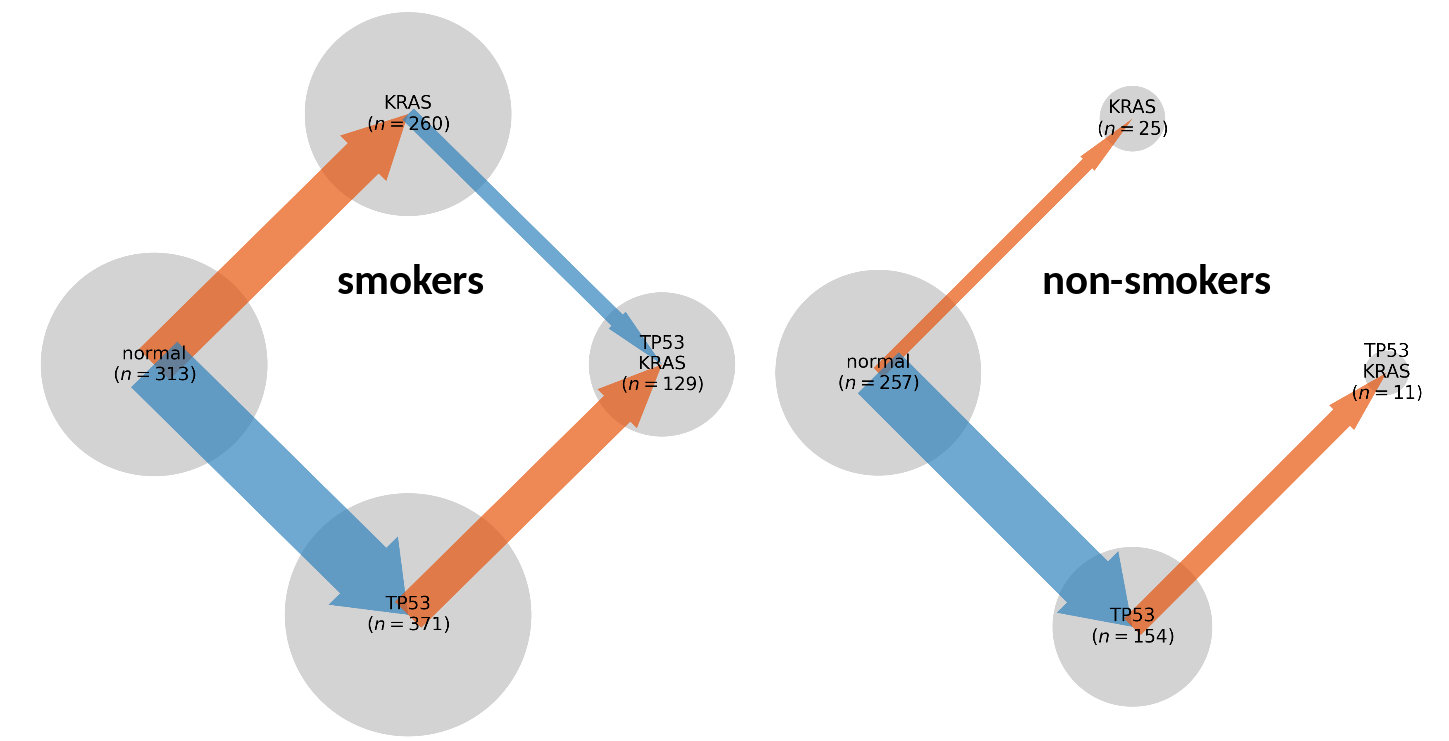
\includegraphics[height=2.4in]{tp53_kras}
\end{frame}


\begin{frame}
  \frametitle{Epistasis of \textit{TP53}, \textit{KRAS} and \textit{EGFR}}
    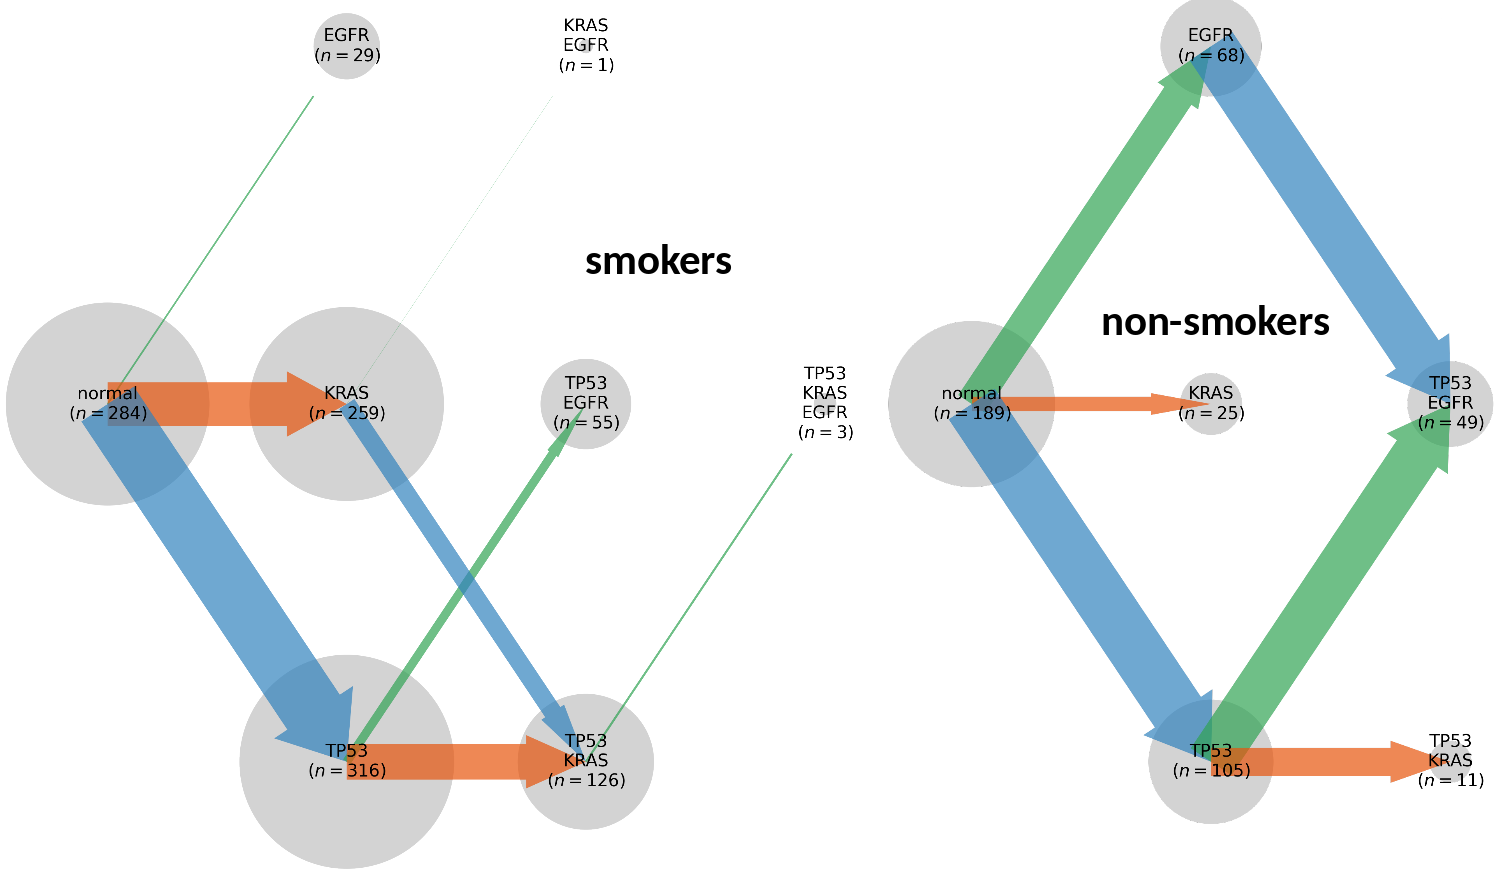
\includegraphics[height=2.4in]{tp53_kras_egfr}
\end{frame}

\begin{frame}
  \frametitle{Epistasis other genes with \textit{TP53}+\textit{KRAS}}
  \begin{center}
    \textbf{non-smokers}
  \end{center}
    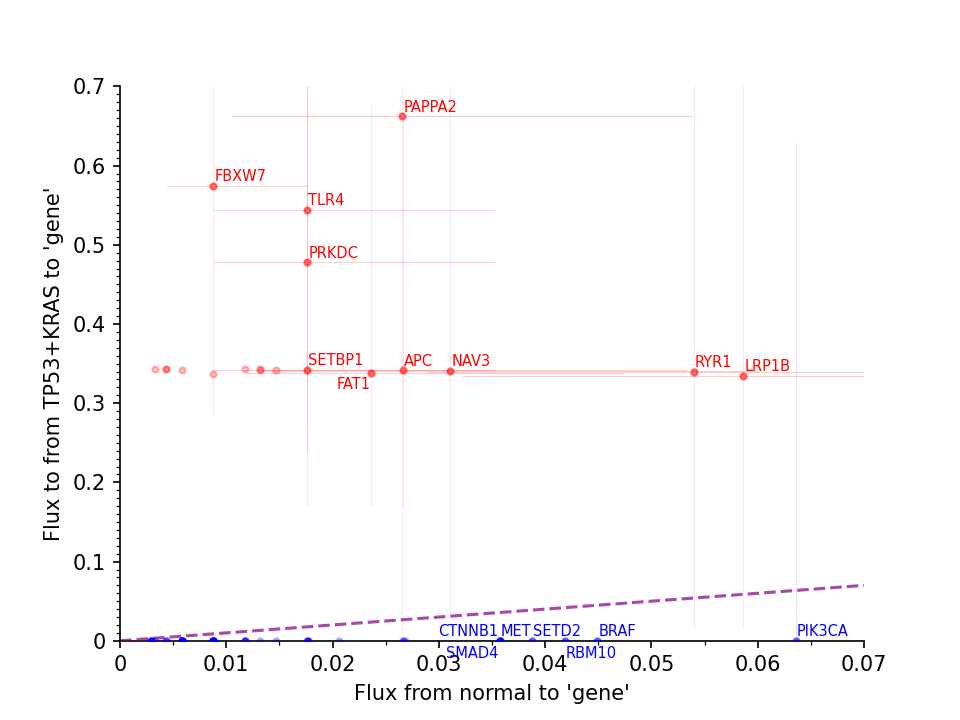
\includegraphics[height=2.8in]{lambdas_from_normal_nonsmoking_plus_vs_lambdas_from_110_nonsmoking_plus}
\end{frame}

\begin{frame}
  \frametitle{Epistasis other genes with \textit{TP53}+\textit{KRAS}}

  \begin{center}
    \textbf{smokers}
  \end{center}
    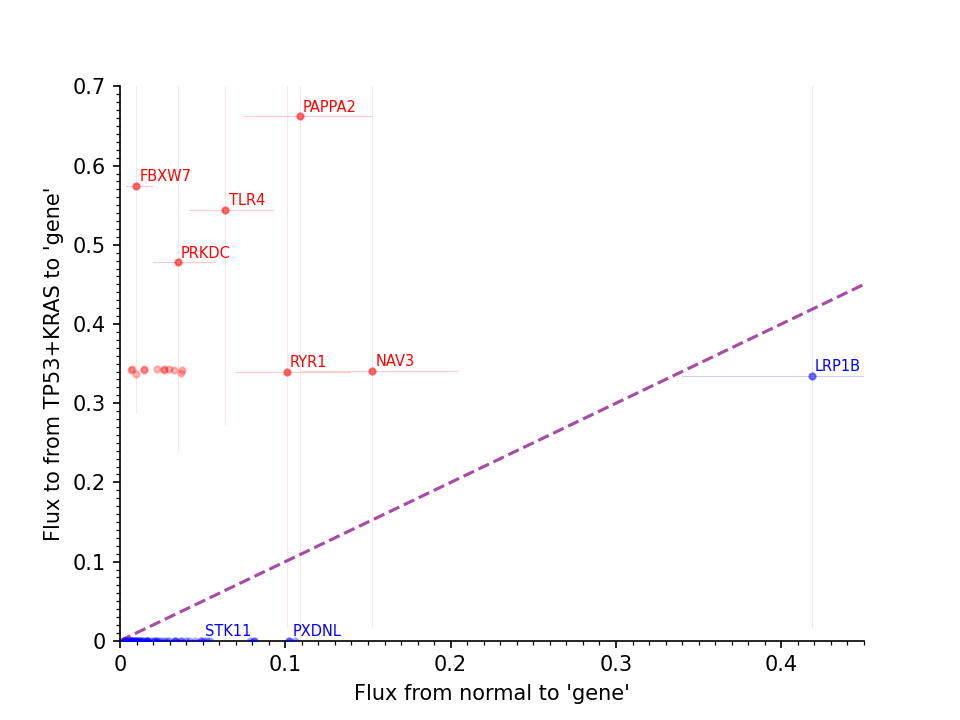
\includegraphics[height=2.8in]{lambdas_from_normal_smoking_plus_vs_lambdas_from_110_smoking_plus}
\end{frame}



% \begin{frame}
%   \frametitle{Future work}
%   \begin{itemize+}
%   \item From flux to mutation rate \& selection
%   \item Time dependency (stages? age?)
%   \item \tt{jorge.alfaro-murillo@yale.edu}
%   \end{itemize+}
% \end{frame}


\end{document}

%%% Local Variables:
%%% mode: latex
%%% TeX-master: t
%%% End:
